%

\documentclass{book}
\usepackage[UTF8]{ctex}
\usepackage{fontspec}
%\usepackage{xeCJK}
\newCJKfontfamily\mincho{IPAexMincho}
\setCJKmainfont{SimSun}[ItalicFont=KaiTi, BoldFont=SimHei]

% SimSun
% STSong
% SimHei
% KaiTi
% DengXian

\def\topos{意象}
\def\nlab{$n$Lab}
\def\regular{常理}
\def\coherent{贯理}
\def\cohesive{凝集}
\def\cohesion{凝集}

\newcommand{\tomeun}{{卷 1 }}

\title{\textbf{\huge 盲人摸象 ($\infty$)}\\\emph{$\infty$-\topos{}理论讲义}}
\author{\emph{王进一}\\\href{我的邮箱}{jin12003@163.com}\\QQ 2917905525}
\date{2024 年夏至今\\~\\~此版本编译时间: \today{}~\\~\\这是一本正在施工的讲义. 目前我迫切需要读者的意见!
	\\~\\
	%在非正式版本中, 我故意将 topos 译为 ``\topos{}''.
}

\usepackage{amsthm}
\usepackage{amsmath}
\usepackage{amssymb}
\usepackage{mathrsfs}
\usepackage{hyperref}
\usepackage{stmaryrd}

%\usepackage{wrapfig}

\usepackage{epigraph}

\usepackage{tikz}
\usetikzlibrary{cd}
\usetikzlibrary{decorations.pathmorphing}

\usepackage{enumerate}

\setcounter{secnumdepth}{1}
\setcounter{tocdepth}{1}

% 哲思

\newcommand{\philoquote}[2]{
	~\\
	\begin{center}
		\begin{minipage}{0.7\linewidth}
			{\quad\sffamily #1}\\
			\begin{flushright}
				\textsf{#2}
			\end{flushright}
		\end{minipage}
	\end{center}
	~\\
}

% 彩色方框


% 彩色方框, 参数的使用有点意思
% 这是打印版的参数 (用于省墨)

\usepackage{tcolorbox}

\tcbuselibrary{breakable}

\newcommand{\framecolor}{gray!50!white}

\newtcolorbox[
auto counter,
number within=section,
]{remark}[2][]{
	colback=white,
	colbacktitle=white,
	colframe=\framecolor,
	coltitle=black,
	breakable,
	title={\textsf{注~\thetcbcounter} #2},
	#1
}

\def\examplecolor{white}
\newtcolorbox[
use counter from=remark,
%number within=chapter,
]{example}[2][]{
	colback=white,
	colbacktitle=white,
	colframe=\framecolor,
	coltitle=black,
	breakable,
	title={\textsf{例~\thetcbcounter} #2},
	#1
}
\newtcolorbox[
use counter from=remark,
%number within=chapter,
]{definition}[2][]{
	colback=white,
	colbacktitle=white,
	colframe=\framecolor,
	coltitle=black,
	breakable,
	title={\textsf{定义~\thetcbcounter} #2},
	#1
}

\def\propcolor{white}
\newtcolorbox[
use counter from=remark,
]{prop}[2][]{
	colback=white,
	colbacktitle=white,
	colframe=\framecolor,
	coltitle=black,
	breakable,
	title={\textsf{命题~\thetcbcounter} #2},
	#1
}
\newtcolorbox[
use counter from=remark,
]{propdef}[2][]{
	colback=white,
	colbacktitle=white,
	colframe=\framecolor,
	coltitle=black,
	breakable,
	title={\textsf{命题-定义~\thetcbcounter} #2},
	#1
}

\newtcolorbox[
auto counter,
number within=chapter
]{exercise}[2][]{
	colback=white,
	colbacktitle=white,
	colframe=\framecolor,
	coltitle=black,
	title={\textsf{习题~\alph{\thetcbcounter}} #2},
	#1
}
\newtcolorbox[
use counter from=remark,
]{axiom}[2][]{
	colback=white,
	colbacktitle=white,
	colframe=\framecolor,
	coltitle=black,
	title={\textsf{公理~\thetcbcounter} #2},
	#1
}

% 分栏
\usepackage{multicol}

% 页边距
\usepackage{geometry}
\geometry{
	b5paper,
	left=15mm,
	right=15mm,
	top=20mm,
	bottom=20mm
}
%\renewcommand{\baselinestretch}{0.9}

% 页眉与页脚样式
\usepackage{fancyhdr}

\newcommand{\chaptert}{}
\newcommand{\sectiont}{}

\renewcommand{\chaptermark}[1]{\renewcommand{\chaptert}{第\ \thechapter\ 章\ #1}}
\renewcommand{\sectionmark}[1]{\renewcommand{\sectiont}{\thesection\ #1}}

\fancypagestyle{plain}{
	\fancyhf{}
	\renewcommand{\headrulewidth}{0pt}
	\renewcommand{\footrulewidth}{0pt}
	\fancyfoot[LE,RO]{\thepage}
}

\fancypagestyle{Jfancy}{
	\fancyhead[LE]{\chaptert{}}
	\fancyhead[RO]{\sectiont{}}
	\fancyhead[RE,LO]{}
	\fancyfoot[C]{}
	\fancyfoot[LE,RO]{\thepage}
	\renewcommand{\headrulewidth}{0.4pt}% Line at the header visible
	\renewcommand{\footrulewidth}{0pt}% Line at the footer visible
}

\pagestyle{Jfancy}

% 参考文献
\usepackage{biblatex}
\addbibresource{infty-topos.bib}

% 跨文档引用 (引用第一卷)
\usepackage{xr}
\externaldocument[t1-]{topos}

% 章节样式
\usepackage{titlesec}
\titleformat{\chapter}{\huge\bfseries}{第\, \thechapter\, 章}{1em}{}

\usepackage{minitoc}
\renewcommand{\mtctitle}{}

\usepackage{multirow}

% 常用记号

\newcommand{\op}{\text{op}} % 对偶范畴
\newcommand{\yo}{\!\text{{\mincho よ}}} % 米田嵌入
\newcommand{\Top}{\mathcal T\hspace{-3pt}opos}
\newcommand{\interpretation}[1]{{[\![#1]\!]}}
\newcommand{\upward}[1]{\uparrow{\!}{#1}}

% sequent calculus
\newcommand{\sqc}[2]{\dfrac{\quad #1 \quad}{\quad #2 \quad}}
\newcommand{\sqqc}[2]{
	\begin{array}
		{c}
		#1 \\ \hline \hline #2
	\end{array}
}

\newcommand{\todo}[1]{{\color{red} [\textbf{未完成: #1}]}}
\newcommand{\internalprop}[1]{{\ulcorner {#1} \urcorner}}

\begin{document}
	\dominitoc
	
	\maketitle
	
	\tableofcontents
	
	\setcounter{chapter}{-1} % 这样下面一章就是第 0 章
	
	% 第零章 前言
	\chapter{前言}

本书是\topos{}理论讲义 ``盲人摸象'' 的续篇, 讲述 $\infty$-\topos{}理论, 即\topos{}理论的 $\infty$-范畴版本.




范畴论的大部分内容 (包括\topos{}理论) 都有在 $\infty$-范畴中的类比, 但后者包含许多新的现象, 这些新内容是本书的重点.



	
	\chapter{$\infty$-范畴的语言}

% 简要介绍无穷范畴的历史?

\philoquote{The traditional way in the literature to provide foundations (for higher category theory) is via the theory of \emph{quasi-categories}, which in turn rests on set theory. While this can be done, the language of set theory is simply not very adequate to model homotopical notions, ...}{Denis-Charles Cisinski, \cite{FHC}}

%像许多 $\infty$-范畴论的文献一样, 本书使用 $\infty$-范畴的一种公理化语言. 我们不是从 $\infty$-范畴的任何一种定义 (或模型) 出发, 而是以公理的形式刻画期望中 $\infty$-范畴的行为. %这样我们可以获得\emph{模型无关} (model-independent) 的结果.



%同伦类型论 (Homotopy Type Theory, HoTT) 提供了 $\infty$-群胚的语言. 我们也可以用一种类似的类型论来谈论 $\infty$-范畴.
% https://arxiv.org/pdf/1705.07442

$\infty$-范畴作为一种模糊的概念已经存在很久. 然而在数学上, $\infty$-范畴没有确切的定义. 在集合论的基础上, 为了逼近心目中那个完美的概念, 人们建立了 $\infty$-范畴各种各样的\emph{模型}. 最著名的模型是由 Andr\'e Joyal 提出, Jacob Lurie \cite{HTT} 发展的基于单纯集的\emph{拟范畴} (quasicategory). 每一种模型都有人为的成分, 而模型之间的等价性是非常不平凡的问题. %在模型中手动构造任何函子都是几乎不可能的.

设想有一个称为 ``\emph{无穷范畴国}'' 的天国乐园, 其国民使用 $\infty$-范畴内蕴的语言作为母语, 他们谈笑之间就可以完成凡人不可想象的工作. 在地上, 说着集合论语言的人们用尽力气, 搭建了通往天国的阶梯, 到访了天国. 但人们发现, 为了理解无穷范畴中任何一件稀松平常的小事, 都要耗费数倍的精力. 地上的人们终于意识到, 语言不通是他们面前最大的阻碍. 要想像母语者那样自如地使用无穷范畴, 就必须抛弃集合论的某些思维, 甚至经典逻辑的一些信条.

能代替集合论成为数学基础, 并且适合于 $\infty$-范畴理论的一种语言是\emph{同伦类型论} (homotopy type theory, HoTT) \cite{hottbook}, 同伦类型论以基本概念 ``类型'' 为 $\infty$-群胚提供了语法, 并且自身包含了一整套推理系统; 理解这种语言对理解 $\infty$-范畴理论中的许多现象有很大的帮助, 因此我们在第 0 节简要介绍之. Emily Riehl 与 Michael Shulman \cite{riehl2023typetheorysyntheticinftycategories} 使用 HoTT 的变种 ``有向类型论'' (directed type theory) 建立了一种综合 $\infty$-范畴理论, Matthew Weaver 和 Daniel Licata 采用的另一变种 ``立方类型论'' (cubical type theory) 也在这个领域展现出一些优势.


%从地上通向天国的阶梯

\setcounter{section}{-1}
\section{同伦类型论基础}

本节介绍的同伦类型论仅供 $\infty$-群胚的理解所需, 因此我们不会使用最正式的语言 (对此有需要的读者可参见 \cite{hottbook} 附录 A).

\begin{axiom}
	{(类型, 对象)}
	同伦类型论有两个基本概念, \emph{类型} (type) 与\emph{对象} (object);
	有一个基本\emph{断言} (judgement)
	\[
	a : A
	\]
	表示 ``对象 $a$ 具有类型 $A$''.
\end{axiom}

\begin{remark}
	{}
	在同伦类型论中, 类型的直观是空间, 而对象是空间中的点.
	此外, \emph{断言}和\emph{命题}是不同的两种东西. 后面我们会介绍命题是一种特殊的类型.
\end{remark}

\begin{axiom}
	{(宇宙)}
	有一个类型 $\mathcal U$ 称为\emph{宇宙},
	我们将用陈述 $$A : \mathcal U$$
	表示 ``$A$ 是类型''.
\end{axiom}

\newcommand{\refl}{\mathsf{refl}}

\begin{axiom}
	{(等式类型)}
	对于类型 $A : \mathcal U$ 的两个对象 $a,b:A$, 有一个类型
	\[
	a=_Ab, \quad\text{或简记为}\quad a=b,
	\]
	称为\emph{等式类型} (identity type).
	
	对每个对象 $a : A$ 有一个对象
	\[
	\refl_a : a=a,
	\]
	称为\emph{自反} (reflexivity).
\end{axiom}

\begin{remark}
	{}
	在同伦类型论中, 两个对象的相等不是一个\emph{断言}, 也不是一个\emph{命题}, 而是一个新的\emph{类型}.
	这就如同一个空间中两个点之间的道路构成一个新的空间,
	又如同 $\infty$-群胚中两个对象之间的态射构成一个新的 $\infty$-群胚;
	这个新的类型包含的同伦信息不止于空或非空.
	
	有时我们也需要以断言的形式表达两个对象依定义相等. 请注意等式类型与依定义相等的区别.
\end{remark}

\begin{axiom}
	{(依定义相等)}
	同伦类型论有一个基本断言
	\[
	a\equiv b : A
	\]
	表示 ``类型 $A$ 的两个对象 $a$ 与 $b$ 依定义相等''.
\end{axiom}

\begin{axiom}
	{(函数类型)}
	对于两个类型 $A,B : \mathcal U$, 有一个类型 $$(A\to B) : \mathcal U,$$
	称为\emph{函数类型} (function type).
	对 $f\colon A\to B$ 以及 $a : A$ 有 $f(a) : B$.
	
	对于含有变量 $x$ 的表达式 $\Phi$, 若 $x : A$ 时有 $\Phi : B$,
	则可定义所谓 \emph{$\lambda$-抽象} (abstraction)
	\[
	(\lambda x.\Phi) : A \to B,
	\]
	此时对于 $a : A$, 记 $\Phi'$ 为将表达式 $\Phi$ 中所有 $x$ 替换为 $a$ 的结果,
	则有
	$$(\lambda x.\Phi)(a) \equiv \Phi'.$$
	对每个 $f \colon A\to B$ 有
	$$
	f \equiv (\lambda x.f(x)).
	$$
\end{axiom}

\begin{example}
	{(依值类型)}
	一个函数 $B\colon A \to \mathcal U$ 称作一个\emph{类型族} (type family) 或一族\emph{依值类型} (dependent type),
	即对类型 $A$ 的每个对象 $a : A$ 都有一个类型 $B(a) : \mathcal U$.
\end{example}

\newcommand{\pr}{\mathsf{pr}}

\begin{axiom}
	{(乘积类型)}
	对于两个类型 $A,B : \mathcal U$ 有一个类型 $$(A\times B) : \mathcal U,$$
	称为\emph{乘积类型} (product type),
	其对象形如 $(a,b)$, $a:A$, $b:B$.
	有两个函数 $$\pr_1\colon A\times B\to A,\quad
	\pr_2\colon A\times B\to B,$$
	以及断言
	\[
	\pr_1((a,b)) \equiv a,\quad
	\pr_2((a,b)) \equiv b.
	\]
\end{axiom}

\begin{axiom}
	{(依值和类型)}
	对于类型 $A : \mathcal U$ 以及依值类型 $B : A \to \mathcal U$,
	有一个类型
	\[
	\sum_{x : A} B(x),
	\]
	称为\emph{依值和类型} (dependent sum type),
	其对象形如 $(a,b)$, $a:A$, $b:B(a)$.
	有一个函数 $$\pr_1\colon \Big(\sum_{x : A} B(x)\Big) \to A.$$
\end{axiom}

\begin{axiom}
	{(依值积类型)}
	对于类型 $A : \mathcal U$ 以及依值类型 $B : A \to \mathcal U$,
	有一个类型
	\[
	\prod_{x : A} B(x),
	\]
	称为\emph{依值积类型} (dependent product type),
	对于表达式 $\Phi : B(x)$,
	有 $$\lambda x.\Phi : \prod_{x:A} B(x).$$
	对于 $f:\prod_{x:A} B(x)$ 以及 $a:A$ 有 $f(a) : B(a)$, 且有断言
	$f(a) \equiv \Phi'$, $\Phi'$ 为将 $\Phi$ 中所有 $x$ 替换为 $a$ 得到的表达式.
\end{axiom}



\begin{definition}
	{(命题是类型)}
	同伦类型论中的\emph{命题}是\emph{类型}.
	证明一个命题就是构造一个类型的对象.
	\begin{center}
		\begin{tabular}{ll}
			命题 & 类型 \\
			\hline
			$A$ 且 $B$ & $A\times B$ \\
			$A$ 或 $B$ & $A+B$\\
			若 $A$ 则 $B$ & $A\to B$\\
			非 $A$ & $A\to 0$\\
			$A$ 当且仅当 $B$ & $(A\to B)\times (B\to A)$\\
			对任意 $x:A$, $P(x)$ & $\prod_{x:A}P(x)$\\
			存在 $x:A$, $P(x)$ & $\sum_{x : A} P(x)$
		\end{tabular}
	\end{center}
\end{definition}

\subsection{集合, 逻辑与截断性}

\newcommand{\isprop}{\mathsf{isProp}}
\newcommand{\isset}{\mathsf{isSet}}
\newcommand{\iscontr}{\mathsf{isContr}}

\begin{definition}
	{(命题)}
	对于类型 $P$ 定义
	\[
	\isprop(P) :\equiv \prod_{x,y : P} (x=y).
	\]
	若 $\isprop(P)$ 有对象, 则称 $P$ 为\emph{命题}.
\end{definition}

\begin{remark}
	{(排中律)}
	在同伦类型论中, 排中律可定义为
	\[
	\mathsf {LEM} :\equiv \prod_{A : \mathcal U}\big(
	\isprop(A) \to (A + \neg A)
	\big).
	\]
	构造主义告诉我们许多的数学不需要排中律 (但这不代表我们需要否认排中律).
\end{remark}

\begin{definition}
	{(集合)}
	对于类型 $S$ 定义
	\[
	\isset(S) :\equiv \prod_{x,y : S}\isprop(x=y).
	\]
	若 $\isset(S)$ 有对象, 则称 $S$ 为\emph{集合}.
\end{definition}

\begin{definition}
	{(命题截断)}
	对于类型 $A$ 有一个类型 $\|A\|$, 称为其\emph{命题截断} (propositional truncation),
	\begin{itemize}
		\item 对任意 $a:A$ 有 $|a|:\|A\|$;
		\item 对任意 $x,y:\|A\|$ 有 $x=y$.
	\end{itemize}
\end{definition}

\begin{definition}
	{(可缩类型)}
	对于类型 $A$ 定义
	\[
	\iscontr(A) :\equiv \sum_{a : A} \prod_{x : A} (a=x).
	\]
\end{definition}

\begin{remark}
	{}
	按朴素的理解, $\iscontr(A)$ 似乎表达的是连通性: ``存在点 $a:A$, 使得对任意点 $x:A$, 都有一条 $a$ 到 $x$ 的路径.''
	但在同伦类型论中, 依值积类型 (全称量词) 的证据需要某种连续性, 直观上需要这条 $a$ 到 $x$ 的路径随 $x$ ``连续变化'', 于是整个命题描述的就不仅是连通性, 而是可缩性.
\end{remark}

\section{基本概念}

本章不会给出无穷范畴的定义. 相反, 我们描述在无穷范畴的语言中, \emph{我们希望能说什么}, 并以公理的形式刻画期望中 $\infty$-范畴的行为. 请注意本章介绍的不是一个完整的 $\infty$-范畴理论, 这些公理不一定出现在最终 ``完美'' 的理论中, 甚至我们不知道那样一个理论是否存在或唯一.

\begin{axiom}
	{($\infty$-范畴)}
	我们要谈论一些对象, 称之为 \emph{$\infty$-范畴} $\mathcal C,\mathcal D,\mathcal E,\cdots$.
	我们还要谈论这些对象之间的\emph{函子} $f\colon \mathcal C\to \mathcal D$, $g\colon \mathcal D\to\mathcal E$ 等等.
\end{axiom}

% 无穷范畴的等价是什么? 伴随等价还是朴素等价?

% 要不要先描述无穷群胚? 我觉得是合理的, 按照 r 递增的顺序来描述 (∞,r)-范畴.

% 澄清 "唯一" 的概念.

\begin{axiom}
	{(一些重要的 $\infty$-范畴)}
	存在如下的 $\infty$-范畴:
	\begin{itemize}
		\item \emph{始 $\infty$-范畴}, 记作 $0$ (或 $\varnothing$), 满足从 $0$ 到任何 $\infty$-范畴 $\mathcal C$ 有唯一的函子;
		\item \emph{终 $\infty$-范畴}, 记作 $1$, 满足从任何 $\infty$-范畴 $\mathcal C$ 到 $1$ 有唯一的函子;
		\item 对任何两个 $\infty$-范畴 $\mathcal C,\mathcal D$, 存在两者的\emph{积} $\mathcal C\times \mathcal D$,
		使得对另一个 $\infty$-范畴 $\mathcal E$,
		一个函子 $\mathcal E\to\mathcal C\times\mathcal D$ 等同于两个函子 $\mathcal E\to\mathcal C$, $\mathcal E\to\mathcal D$;
		\item 对任何两个 $\infty$-范畴 $\mathcal C,\mathcal D$, 存在两者的\emph{和} $\mathcal C + \mathcal D$,
		使得对另一个 $\infty$-范畴 $\mathcal E$,
		一个函子 $\mathcal C + \mathcal D \to \mathcal E$ 等同于两个函子 $\mathcal C \to \mathcal E$, $\mathcal D \to \mathcal E$;
		\item 对任何两个 $\infty$-范畴 $\mathcal C,\mathcal D$, 有\emph{函子范畴} $\mathsf {Fun}(\mathcal C,\mathcal D)$,
		也记作 $\mathcal D^{\mathcal C}$, 使得对另一个 $\infty$-范畴 $\mathcal E$,
		函子 $\mathcal E\to \mathcal D^{\mathcal C}$ 等同于函子 $\mathcal E\times\mathcal C \to \mathcal D$;
	\end{itemize}
\end{axiom}

\begin{axiom}
	[label={regular-category-as-infinity-category}]
	{($1$-范畴视为 $\infty$-范畴)}
	每个普通范畴 (即 $1$-范畴) 都可以视为 $\infty$-范畴. 普通范畴之间的函子也可以视为对应的 $\infty$-范畴之间的函子.
	普通范畴的和与积就是它们作为 $\infty$-范畴的和与积.
\end{axiom}

\begin{axiom}
	{(对象, 态射)}
	$\infty$-范畴 $\mathcal C$ 的\emph{对象}等同于函子 $1\to \mathcal C$.
	两个对象之间的态射等同于函子 $\{*\to *\}\to \mathcal C$, 其中 $\{*\to *\}$ 视为 $\infty$-范畴 (公理 \ref{regular-category-as-infinity-category}).
	称函子范畴 $\mathcal C^{\{*\to *\}}$ 为\emph{箭头范畴}, 也简记为 $\mathcal C^\rightarrow$.
\end{axiom}

\section{$\infty$-范畴中的结构与性质}

\subsection{连通性与截断性}

% HoTT?

\begin{definition}
	{($n$-截断 $\infty$-群胚, $n$-群胚)}
	设 $n\geq -1$ 为整数. 称一个 $\infty$-群胚 $X$  \emph{$n$-截断} (或称其为 \emph{$n$-群胚}) 是指其所有大于 $n$ 阶的同伦群 $\pi_k(X)\,(k>n)$ 均平凡.
\end{definition}

\begin{definition}
	{($n$-群胚, 等价定义)}
	设 $n\geq -1$ 为整数. 称一个 $\infty$-群胚 $X$  \emph{$n$-截断}是指 $X$ 为关于 $\{S^{n+1}\to *\}$ 的局部对象.
\end{definition}

\begin{example}
	{(低维群胚的例子)}
	在同伦等价的意义下,
	\begin{itemize}
		\item $(-2)$-群胚是一个点.
		\item $(-1)$-群胚是空集或一个点.
		\item $0$-群胚是集合, 也即离散群胚.
	\end{itemize}
\end{example}

\subsection{$n$-范畴}

\begin{definition}
	[label={local-objects-infinity-category}]
	{(局部对象)}
	设 $\mathcal C$ 为 $\infty$-范畴, $S$ 为 $\mathcal C$ 中一族态射的集合, 称 $\mathcal C$ 的对象 $x$ 为 \emph{$S$-局部对象}是指对 $S$ 中任意态射 $f\colon a\to b$,
	\[
	f^*\colon \operatorname{Hom}_{\mathcal C}(b,x) \to \operatorname{Hom}_{\mathcal C}(a,x)
	\]
	为 $\infty$-群胚的等价.
	%这是定义 \ref{local-objects} 在 $\infty$-范畴中的类比.
\end{definition}

\begin{definition}
	{(球面)}
	归纳定义 $\infGpdinfcat$ 的 \emph{$n$ 维球面} $S^n\,(n\geq -1)$ 如下:
	\begin{itemize}
		\item $S^{-1}=\varnothing$;
		\item 对 $n\geq -1$, $S^{n+1}$ 是如图所示的推出.
		% https://q.uiver.app/#q=WzAsNCxbMCwwLCJTXntufSJdLFswLDEsIioiXSxbMSwwLCIqIl0sWzEsMSwiU157bisxfSJdLFswLDFdLFsxLDNdLFswLDJdLFsyLDNdXQ==
	\end{itemize}
	\vspace{-6.5em}
	\begin{flushright}
		$\begin{tikzcd}[ampersand replacement=\&,column sep=small]
			{S^{n}} \& {*} \\
			{*} \& {S^{n+1}}
			\arrow[from=1-1, to=2-1]
			\arrow[from=2-1, to=2-2]
			\arrow[from=1-1, to=1-2]
			\arrow[from=1-2, to=2-2]
		\end{tikzcd}$
	\end{flushright}
\end{definition}

\begin{definition}
	{($n$-群胚)}
	对整数 $n\geq -2$, 定义 \emph{$n$-群胚}为 $\infGpdinfcat$ 中关于 $\{S^{n+1}\to *\}$ 的局部对象 (定义 \ref{local-objects-infinity-category}).
\end{definition}



\subsection{东西, 结构, 性质}

\subsection{伴随}

%在定义极限和余极限之前, 我们需要指出 $\infty$-范畴之间的伴随. 注意以下陈述是模型无关的.

\begin{definition}
	{($\infty$-范畴之间的伴随)}
	$\infty$-范畴之间的一对伴随 \begin{tikzcd}[ampersand replacement=\&]
		{\mathcal D} \& {\mathcal C}
		\arrow[""{name=0, anchor=center, inner sep=0}, "F"', shift right=2, from=1-2, to=1-1]
		\arrow[""{name=1, anchor=center, inner sep=0}, "G"', shift right=2, from=1-1, to=1-2]
		\arrow["\dashv"{anchor=center, rotate=-90}, draw=none, from=0, to=1]
	\end{tikzcd}
	是如下资料,
	\begin{itemize}
		\item 两个 $\infty$-范畴 $\mathcal C,\mathcal D$,
		\item 两个函子 $F\colon \mathcal C\to \mathcal D$ (称为\emph{左伴随}), $G\colon \mathcal D\to \mathcal C$ (称为\emph{右伴随}),
		\item 两个自然变换 $\eta\colon \operatorname{id}_{\mathcal C}\to GF$ (称为\emph{单位}), $\varepsilon\colon FG\to\operatorname{id}_{\mathcal D}$ (称为\emph{余单位});
	\end{itemize}
	满足如下 $2$-态射的关系,
	\[\begin{tikzcd}[ampersand replacement=\&,column sep=1.5em]
		{\mathcal C} \&\& {\mathcal C} \\
		\& {\mathcal D} \&\& {\mathcal D}
		\arrow["F"', from=1-1, to=2-2]
		\arrow["G"{description}, from=2-2, to=1-3]
		\arrow["F", from=1-3, to=2-4]
		\arrow[""{name=0, anchor=center, inner sep=0}, "{\operatorname{id}_{\mathcal C}}", from=1-1, to=1-3]
		\arrow[""{name=1, anchor=center, inner sep=0}, "{\operatorname{id}_{\mathcal D}}"', from=2-2, to=2-4]
		\arrow["\eta"', shorten <=3pt, shorten >=3pt, Rightarrow, from=0, to=2-2]
		\arrow["\varepsilon", shorten <=3pt, shorten >=3pt, Rightarrow, from=1-3, to=1]
	\end{tikzcd}\hspace{-1em}\sim \operatorname{id}_F,
	\begin{tikzcd}[ampersand replacement=\&,column sep=1.5em]
		\& {\mathcal C} \&\& {\mathcal C} \\
		{\mathcal D} \&\& {\mathcal D}
		\arrow["G", from=2-1, to=1-2]
		\arrow["F"{description}, from=1-2, to=2-3]
		\arrow["G"', from=2-3, to=1-4]
		\arrow[""{name=0, anchor=center, inner sep=0}, "{\operatorname{id}_{\mathcal D}}"', from=2-1, to=2-3]
		\arrow[""{name=1, anchor=center, inner sep=0}, "{\operatorname{id}_{\mathcal C}}", from=1-2, to=1-4]
		\arrow["\varepsilon", shorten <=3pt, shorten >=3pt, Rightarrow, from=1-2, to=0]
		\arrow["\eta"', shorten <=3pt, shorten >=3pt, Rightarrow, from=1, to=2-3]
	\end{tikzcd}\hspace{-1em}\sim\operatorname{id}_{G},\]
	其中第一个式子中 $\sim$ 表示 $\operatorname{id}_F$ 是 $\infty$-范畴 $\mathsf {Fun}(\mathcal C,\mathcal D)$ 中两个态射 $F\to FGF$, $FGF\to F$ 的一个复合.
	
	记 $\Ho_2(\infCatinfcat)$ 为 $\infCatinfcat$ 的\emph{同伦 $2$-范畴}, 其中 $\operatorname{Hom}_{\Ho_2(\infCatinfcat)}(\mathcal C,\mathcal D) := \Ho{}(\operatorname{Fun}(\mathcal C,\mathcal D))$. 由定义, $\infty$-范畴之间的伴随等同于 $\Ho_2(\infCatinfcat)$ 中的伴随.
\end{definition}

\begin{prop}
	{($\infty$-范畴之间的伴随与 $\operatorname{Hom}$-函子)}
	设 \begin{tikzcd}[ampersand replacement=\&]
		{\mathcal D} \& {\mathcal C}
		\arrow[""{name=0, anchor=center, inner sep=0}, "F"', shift right=2, from=1-2, to=1-1]
		\arrow[""{name=1, anchor=center, inner sep=0}, "G"', shift right=2, from=1-1, to=1-2]
		\arrow["\dashv"{anchor=center, rotate=-90}, draw=none, from=0, to=1]
	\end{tikzcd} 为 $\infty$-范畴之间的伴随, 则对任意对象 $C\in\mathcal C$, $D\in\mathcal D$, 函子
	\[
	\operatorname{Hom}_{\mathcal D}(F(C),D) \overset{G}{\longrightarrow} \operatorname{Hom}_{\mathcal C}(GF(C),G(D))
	\overset{\eta_C^*}{\longrightarrow}
	\operatorname{Hom}_{\mathcal C}(C,G(D))
	\]
	为\emph{同伦等价}.
\end{prop}

\subsection{极限与余极限}

\begin{definition}
	{(终对象, 始对象)}
	设 $\mathcal C$ 为 $\infty$-范畴, $x$ 为 $\mathcal C$ 中的对象. 若如下等价条件成立,
	则称 $x$ 为 $\mathcal C$ 的\emph{始对象}:
	\begin{itemize}
		\item 对任意对象 $y$, $\operatorname{Hom}_{\mathcal C}(y,x)\simeq 1$;
		\item $x\colon 1\to\mathcal C$ 是 $\mathcal C\to 1$ 的右伴随.
	\end{itemize}
	对偶地定义\emph{始对象}.
	
	%等价的定义是, $\mathcal X$ 的终对象是 (唯一的) 函子 $\mathcal X\to 1$ 的\emph{右伴随} $1\to\mathcal X$, $\mathcal X$ 的始对象是函子 $\mathcal X\to 1$ 的\emph{左伴随} $1\to\mathcal X$; 这告诉我们终对象和始对象的概念实际上存在于 $\infty$-范畴构成的 \emph{$2$-范畴}中, 见例 \ref{terminal-object-2-categorical}.
\end{definition}

\begin{definition}
	{(俯范畴, 仰范畴)}
	设 $\mathcal C$ 为 $\infty$-范畴, $x$ 为 $\mathcal C$ 中的对象. 定义\emph{俯范畴} $\mathcal C/x$ 为如下的拉回:
	% https://q.uiver.app/#q=WzAsNCxbMCwxLCJcXERlbHRhXjAiXSxbMSwxLCJYIl0sWzEsMCwiXFxtYXRoc2Yge0Z1bn0oXFxEZWx0YV4xLFgpIl0sWzAsMCwiWC94Il0sWzAsMSwieCIsMl0sWzIsMSwiMSJdLFszLDBdLFszLDJdXQ==
	\[\begin{tikzcd}[ampersand replacement=\&]
		{{\mathcal C}/x} \& {\mathcal C^{\rightarrow}} \\
		{1} \& {\mathcal X}
		\arrow["x"', from=2-1, to=2-2]
		\arrow["t", from=1-2, to=2-2]
		\arrow[from=1-1, to=2-1]
		\arrow[from=1-1, to=1-2]
	\end{tikzcd}\]
	其中 $t\colon \mathcal C^\rightarrow \to \mathcal C$ 将 ${\mathcal C}$ 的态射对应到其终点.
\end{definition}

由定义, 俯范畴 $\mathcal {\mathcal X}/x$ 的对象是 ${\mathcal X}$ 中以 $x$ 为终点的箭头.
可以说明 $\operatorname{id}_x$ 是 ${\mathcal X}/x$ 的终对象.

\begin{definition}
	{(极限, 余极限)}
	设 $\mathcal C$ 为 $\infty$-范畴, $I$ 为单纯集 (称为\emph{指标集}或\emph{指标范畴}), $F\colon I\to\mathcal C$ 为单纯集映射 (称为 $\mathcal C$ 中的一个\emph{图表}).
	类似于普通范畴中极限的定义, 我们可以构造一个 (广义的) ``俯范畴'' $\mathcal C_{/F}$, 其对象为 $\mathcal C$ 的对象到 $F$ 的锥. 具体地, $\mathcal C_{/F}$ 为如下拉回.
	\[\begin{tikzcd}[ampersand replacement=\&]
		{\mathcal C_{/F}} \& {({\mathcal C}^I)_{/F}} \\
		{\mathcal C} \& {{\mathcal C}^I}
		\arrow["{\text{常值}}"', from=2-1, to=2-2]
		\arrow[from=1-2, to=2-2]
		\arrow[from=1-1, to=2-1]
		\arrow[from=1-1, to=1-2]
	\end{tikzcd}\]
	其中 $\text{``常值''}\colon \mathcal C\simeq\mathcal C^{\Delta^0}\to \mathcal C^I$ 是 $I\to \Delta^0$ 的拉回, 它将 $\mathcal C$ 的对象 $x\colon \Delta^0\to\mathcal C$ 对应到 $x$ 处的 ``常值图表'' $I\to\Delta^0\to\mathcal C$, 就像普通范畴的情形一样.
	定义图 $F$ 的\emph{极限}为 ``俯范畴'' $\mathcal C_{/F}$ 的终对象; 对偶地, 定义 $F$ 的\emph{余极限}为 ``仰范畴'' $\mathcal C_{F/}$ 的始对象.
\end{definition}

\begin{remark}
	{(同伦极限, 同伦余极限)}
	$\infty$-范畴中的极限和余极限与所谓\emph{同伦极限, 同伦余极限}有关.
	
	拓扑空间范畴 $\mathsf {Top}$ 中的极限和余极限不是\emph{同伦不变}的. 例如, 下图 (a) 的推出是 $S^{n+1}$ ($S^n$ 是 $n$ 维球面, $D^{n+1}$ 是 $(n+1)$ 维圆盘, $S^n\to D^{n+1}$ 是圆盘的边界), 将 $D^{n+1}$ 替换为与之同伦等价的一个点 $*$ 得到图 (b), 但 (b) 的推出却不是 $S^{n+1}$, 而是一个点 $*$.
	相比之下, \emph{同伦极限, 同伦余极限}则是同伦不变的概念; 例如 (a), (b) 的同伦推出都是 $S^{n+1}$.
	\[
	\begin{array}
		{ccc}
		\begin{tikzcd}[ampersand replacement=\&,column sep=small]
			{S^{n}} \& {D^{n+1}} \\
			{*} \& {}
			\arrow[from=1-1, to=2-1]
			%\arrow[from=2-1, to=2-2]
			\arrow[from=1-1, to=1-2]
			%\arrow[from=1-2, to=2-2]
		\end{tikzcd} & \begin{tikzcd}[ampersand replacement=\&,column sep=small]
			{S^{n}} \& {*} \\
			{*} \& {}
			\arrow[from=1-1, to=2-1]
			%\arrow[from=2-1, to=2-2]
			\arrow[from=1-1, to=1-2]
			%\arrow[from=1-2, to=2-2]
		\end{tikzcd} & \begin{tikzcd}[ampersand replacement=\&,column sep=small]
			{A} \& {X} \\
			{Y} \& {}
			\arrow["g"',from=1-1, to=2-1]
			%\arrow[from=2-1, to=2-2]
			\arrow["f",from=1-1, to=1-2]
			%\arrow[from=1-2, to=2-2]
		\end{tikzcd}\\
		\text{(a)} & \text{(b)} & \text{(c)}
	\end{array}
	\]
	对一般的两个映射 $f\colon A\to X$, $g\colon A\to Y$, 以 $\mathbb I$ 表示单位区间 $[0,1]$, 图 (c) 的同伦推出可构造为商空间
	$$
	X \sqcup (A\times \mathbb I) \sqcup Y \Big/ \sim,\quad\text{其中}\quad
	(a,0)\sim f(a), (a,1)\sim g(a).
	$$
	%	它也可表示为
	%	$$
	%	\operatorname{coeq}\Big[
	%	A\times [0,1] \rightrightarrows \Big(X \sqcup  Y\Big)
	%	\Big]
	%	$$
	直观上这是将以 $A$ 为底的柱形两端分别粘到 $X$ 和 $Y$ 上所得的空间. 对于每个点 $a\in A$, 普通的推出粗暴地将 $f(a),g(a)$ 粘在一起, 而同伦推出只是在两者之间连了一条线段. 连一条线段与直接粘起来看似 (在同伦的意义下) 等价, 实则保留了更多的信息: 因为两点之间可连多条线段, 即可\emph{以多种方式}粘在一起.
	\begin{center}
		\tikzset{every picture/.style={line width=0.75pt}} %set default line width to 0.75pt        
		
		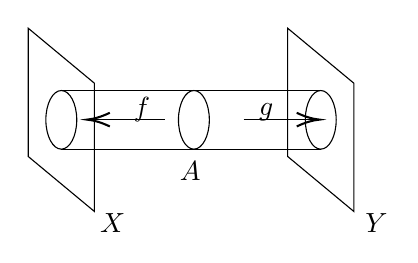
\begin{tikzpicture}[x=0.75pt,y=0.75pt,yscale=-1,xscale=1]
			%uncomment if require: \path (0,300); %set diagram left start at 0, and has height of 300
			
			%Shape: Parallelogram [id:dp15297514694080894] 
			\draw   (96.58,101.28) -- (96.58,163.07) -- (64.71,136.59) -- (64.71,74.8) -- cycle ;
			%Shape: Ellipse [id:dp019834245813657114] 
			\draw   (73.2,118.93) .. controls (73.2,111.13) and (76.54,104.81) .. (80.65,104.81) .. controls (84.76,104.81) and (88.09,111.13) .. (88.09,118.93) .. controls (88.09,126.73) and (84.76,133.06) .. (80.65,133.06) .. controls (76.54,133.06) and (73.2,126.73) .. (73.2,118.93) -- cycle ;
			%Shape: Ellipse [id:dp40259616007577415] 
			\draw   (198.2,118.93) .. controls (198.2,111.13) and (201.54,104.81) .. (205.65,104.81) .. controls (209.76,104.81) and (213.09,111.13) .. (213.09,118.93) .. controls (213.09,126.73) and (209.76,133.06) .. (205.65,133.06) .. controls (201.54,133.06) and (198.2,126.73) .. (198.2,118.93) -- cycle ;
			%Shape: Parallelogram [id:dp06847355000424948] 
			\draw   (221.58,101.28) -- (221.58,163.07) -- (189.71,136.59) -- (189.71,74.8) -- cycle ;
			%Straight Lines [id:da049979386851016994] 
			\draw    (80.65,104.81) -- (205.65,104.81) ;
			%Straight Lines [id:da5162984256492849] 
			\draw    (80.65,133.06) -- (205.65,133.06) ;
			%Shape: Ellipse [id:dp7242785411673776] 
			\draw   (137.09,118.93) .. controls (137.09,111.13) and (140.42,104.81) .. (144.53,104.81) .. controls (148.64,104.81) and (151.97,111.13) .. (151.97,118.93) .. controls (151.97,126.73) and (148.64,133.06) .. (144.53,133.06) .. controls (140.42,133.06) and (137.09,126.73) .. (137.09,118.93) -- cycle ;
			%Straight Lines [id:da2856334310702111] 
			\draw    (130.5,118.83) -- (95.08,118.83) ;
			\draw [shift={(93.08,118.83)}, rotate = 360] [color={rgb, 255:red, 0; green, 0; blue, 0 }  ][line width=0.75]    (10.93,-3.29) .. controls (6.95,-1.4) and (3.31,-0.3) .. (0,0) .. controls (3.31,0.3) and (6.95,1.4) .. (10.93,3.29)   ;
			%Straight Lines [id:da6963451965198226] 
			\draw    (168.5,118.83) -- (203,118.83) ;
			\draw [shift={(205,118.83)}, rotate = 180] [color={rgb, 255:red, 0; green, 0; blue, 0 }  ][line width=0.75]    (10.93,-3.29) .. controls (6.95,-1.4) and (3.31,-0.3) .. (0,0) .. controls (3.31,0.3) and (6.95,1.4) .. (10.93,3.29)   ;
			
			% Text Node
			\draw (136.53,138) node [anchor=north west][inner sep=0.75pt]   [align=left] {$\displaystyle A$};
			% Text Node
			\draw (98.13,163) node [anchor=north west][inner sep=0.75pt]   [align=left] {$\displaystyle X$};
			% Text Node
			\draw (225.93,163) node [anchor=north west][inner sep=0.75pt]   [align=left] {$\displaystyle Y$};
			% Text Node
			\draw (114.25,107) node [anchor=north west][inner sep=0.75pt]   [align=left] {$\displaystyle f$};
			% Text Node
			\draw (174.75,110) node [anchor=north west][inner sep=0.75pt]   [align=left] {$\displaystyle g$};
		\end{tikzpicture}
	\end{center}
	
	同伦推出的例子可以启发一般的同伦余极限. 设 $T\colon I\to \mathsf {Top}$ 为拓扑空间的图表. 对指标范畴 $I$ 每个长为 $n$ 的态射链 $i_0\to i_1\to\cdots\to i_n$, 以及每个点 $a\in T(i_0)$, 普通的余极限会粗暴地将 $a$ 经过这些映射所到的每个点粘在一起, 而同伦余极限则是在这些点之间连上一个拓扑 $n$-单形 $|\Delta^n|$.
	具体地, 先由 $T$ 构造一个自然的单纯空间
	$\mathsf s T\colon \Delta^{\op} \to\mathsf {Top}$, 使得 $$\mathsf s T_n = \coprod_{i_0\to i_1\to\cdots\to i_n} T(i_0).$$
	对于单纯空间 $X\colon \Delta^{\op} \to\mathsf {Top}$, 定义其\emph{几何实现}为如下的余等化子,
	$$
	|X|:= \operatorname{coeq}\Big[
	\coprod_{[n]\to [k]} X_k\times |\Delta^n|
	\rightrightarrows
	\coprod_{n}X_n\times |\Delta^n|
	\Big]
	$$
	其中两个映射分别为
	$$
	\begin{aligned}
		\coprod_{\sigma\colon  [n] \to [k]}& (\sigma^*\colon X_k \to X_n)\times |\Delta^n|,\\
		\coprod_{\sigma\colon  [n] \to [k]}& X_k\times (|\sigma|\colon |\Delta^n|\to |\Delta^k|).
	\end{aligned}
	$$
	那么 $T$ 的\emph{同伦余极限}可构造为
	$$
	\operatorname{hocolim}T := |\mathsf sT|.
	$$
	
	同伦极限的一个例子是同伦拉回. 两个映射 $f\colon X\to A$, $g\colon Y\to A$ 的同伦拉回可构造为 $X\times A^{\mathbb I}\times Y$ 的子空间
	$$
	\big\{ (x,\gamma,y)\in X\times A^{\mathbb I}\times Y\mid  \gamma(0)=f(x),\gamma(1)=g(y)\big\}.
	$$
	同伦拉回中的一个点由 $X$ 的点 $x$, $Y$ 的点 $y$ 以及 $f(x)$ 到 $g(y)$ 的一条道路构成.
	\begin{center}
		\tikzset{every picture/.style={line width=0.75pt}} %set default line width to 0.75pt        
		
		
		\tikzset{every picture/.style={line width=0.75pt}} %set default line width to 0.75pt        
		
		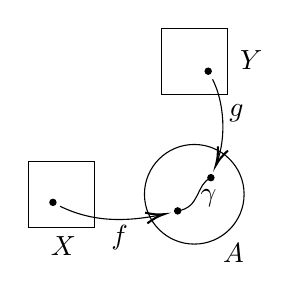
\begin{tikzpicture}[x=0.6pt,y=0.6pt,yscale=-1,xscale=1]
			%uncomment if require: \path (0,300); %set diagram left start at 0, and has height of 300
			
			%Shape: Square [id:dp9029850536154158] 
			\draw   (80,130) -- (120,130) -- (120,170) -- (80,170) -- cycle ;
			%Shape: Square [id:dp04010633466224678] 
			\draw   (160,50) -- (200,50) -- (200,90) -- (160,90) -- cycle ;
			%Shape: Circle [id:dp8217969120991764] 
			\draw   (150,150) .. controls (150,133.43) and (163.43,120) .. (180,120) .. controls (196.57,120) and (210,133.43) .. (210,150) .. controls (210,166.57) and (196.57,180) .. (180,180) .. controls (163.43,180) and (150,166.57) .. (150,150) -- cycle ;
			%Curve Lines [id:da9149134742462921] 
			\draw    (170,160) .. controls (183.75,158) and (180.75,144.25) .. (190,140) ;
			%Shape: Circle [id:dp3191495362532544] 
			\draw  [color={rgb, 255:red, 0; green, 0; blue, 0 }  ,draw opacity=1 ][fill={rgb, 255:red, 0; green, 0; blue, 0 }  ,fill opacity=1 ] (93,154.88) .. controls (93,153.84) and (93.84,153) .. (94.88,153) .. controls (95.91,153) and (96.75,153.84) .. (96.75,154.88) .. controls (96.75,155.91) and (95.91,156.75) .. (94.88,156.75) .. controls (93.84,156.75) and (93,155.91) .. (93,154.88) -- cycle ;
			%Shape: Circle [id:dp6370015580564639] 
			\draw  [color={rgb, 255:red, 0; green, 0; blue, 0 }  ,draw opacity=1 ][fill={rgb, 255:red, 0; green, 0; blue, 0 }  ,fill opacity=1 ] (186.5,75.88) .. controls (186.5,74.84) and (187.34,74) .. (188.38,74) .. controls (189.41,74) and (190.25,74.84) .. (190.25,75.88) .. controls (190.25,76.91) and (189.41,77.75) .. (188.38,77.75) .. controls (187.34,77.75) and (186.5,76.91) .. (186.5,75.88) -- cycle ;
			%Shape: Circle [id:dp21083479803073035] 
			\draw  [color={rgb, 255:red, 0; green, 0; blue, 0 }  ,draw opacity=1 ][fill={rgb, 255:red, 0; green, 0; blue, 0 }  ,fill opacity=1 ] (168.13,160) .. controls (168.13,158.96) and (168.96,158.13) .. (170,158.13) .. controls (171.04,158.13) and (171.88,158.96) .. (171.88,160) .. controls (171.88,161.04) and (171.04,161.88) .. (170,161.88) .. controls (168.96,161.88) and (168.13,161.04) .. (168.13,160) -- cycle ;
			%Shape: Circle [id:dp6826214678369391] 
			\draw  [color={rgb, 255:red, 0; green, 0; blue, 0 }  ,draw opacity=1 ][fill={rgb, 255:red, 0; green, 0; blue, 0 }  ,fill opacity=1 ] (188.13,140) .. controls (188.13,138.96) and (188.96,138.13) .. (190,138.13) .. controls (191.04,138.13) and (191.88,138.96) .. (191.88,140) .. controls (191.88,141.04) and (191.04,141.88) .. (190,141.88) .. controls (188.96,141.88) and (188.13,141.04) .. (188.13,140) -- cycle ;
			%Curve Lines [id:da8630666727441021] 
			\draw    (99.25,157.25) .. controls (118.75,166.76) and (138.49,166.76) .. (160.08,162.35) ;
			\draw [shift={(161.75,162)}, rotate = 167.95] [color={rgb, 255:red, 0; green, 0; blue, 0 }  ][line width=0.75]    (10.93,-3.29) .. controls (6.95,-1.4) and (3.31,-0.3) .. (0,0) .. controls (3.31,0.3) and (6.95,1.4) .. (10.93,3.29)   ;
			%Curve Lines [id:da25052543255059834] 
			\draw    (191,80.75) .. controls (198,94.5) and (199.41,115.47) .. (193.65,130.85) ;
			\draw [shift={(193,132.5)}, rotate = 292.75] [color={rgb, 255:red, 0; green, 0; blue, 0 }  ][line width=0.75]    (10.93,-3.29) .. controls (6.95,-1.4) and (3.31,-0.3) .. (0,0) .. controls (3.31,0.3) and (6.95,1.4) .. (10.93,3.29)   ;
			
			% Text Node
			\draw (195.75,178) node [anchor=north west][inner sep=0.75pt]   [align=left] {$\displaystyle A$};
			% Text Node
			\draw (92,174) node [anchor=north west][inner sep=0.75pt]   [align=left] {$\displaystyle X$};
			% Text Node
			\draw (206,62) node [anchor=north west][inner sep=0.75pt]   [align=left] {$\displaystyle Y$};
			% Text Node
			\draw (128.5,167) node [anchor=north west][inner sep=0.75pt]   [align=left] {$\displaystyle f$};
			% Text Node
			\draw (199.5,94.5) node [anchor=north west][inner sep=0.75pt]   [align=left] {$\displaystyle g$};
			% Text Node
			\draw (182.25,145.75) node [anchor=north west][inner sep=0.75pt]   [align=left] {$\displaystyle \gamma $};
			
			
		\end{tikzpicture}
	\end{center}
	一般地, 设 $T\colon I\to \mathsf {Top}$ 为拓扑空间的图表, 对指标范畴 $I$ 每个长为 $n$ 的态射链 $i_0\to i_1\to\cdots\to i_n$, 以及每个点 $a\in T(i_n)$, 普通的极限只允许 $T(i_0),\cdots,T(i_n)$ 的各点恰好落在 $a$ 上, 而同伦极限允许它们落在 $T(i_n)$ 中的一个 $n$-单形的顶点. 具体地, 构造自然的余单纯空间 $\mathsf cT\colon \Delta \to \mathsf {Top}$, 使得
	$$
	\mathsf cT_n = \prod_{i_0\to \cdots\to i_n} T(i_n).
	$$
	对于余单纯空间 $X\colon \Delta\to\mathsf {Top}$, 定义其\emph{全体} (totalization)\footnotemark{} $\operatorname{Tot}X$ 为如下的等化子,
	$$
	\operatorname{Tot}X := \operatorname{eq}\Big[
	\prod_{n}X_n^{|\Delta^n|}
	\rightrightarrows
	\prod_{[n]\to [k]} X_k^{|\Delta^n|}
	\Big].
	$$
	
	同伦极限和同伦余极限\emph{表现}了 $\infty$-范畴中的极限和余极限. 见 \cite{HTT} 定理 4.2.4.1.
\end{remark}
\footnotetext{几何实现是一种左 Kan 扩张, 而 ``全体'' 是一种右 Kan 扩张. 记 $\mathsf{cosTop}$ 为余单纯空间的范畴, 则余单纯空间 $X$ 的全体也可表示为 $\operatorname{Hom}_{\mathsf{cosTop}}(|\Delta|,X)$, 其中 $|\Delta|\colon \Delta\to \mathsf {Top}$ 将 $[n]$ 对应到拓扑 $n$-单形.}

\begin{example}
	{}
	对于 $I = \varnothing$, 空图表 $F\colon I\to \mathcal C$ 的极限即是 $\mathcal C$ 的终对象.
\end{example}

\begin{example}
	{(推出, 拉回)}
	考虑 $I = \Lambda_2^2$ (见定义 \ref{simplicial-set-horn} 及其后的插图), 则 $F\colon I\to X$ 等同于两个态射 $x\to z$, $y\to z$. 称 $F$ 的极限为 $\infty$-\emph{拉回}, 简称\emph{拉回}, 记为 $x\times_z y$.
	对偶地, 形如 $\Lambda_0^2$ 的图的余极限称为 $\infty$-\emph{推出}, 简称\emph{推出}.
	
	单纯集映射 % https://q.uiver.app/#q=WzAsMyxbMCwwLCJYIl0sWzEsMCwiWSJdLFswLDEsIloiXSxbMCwyXSxbMCwxXV0=
	$\begin{tikzcd}[ampersand replacement=\&,sep=small]
		X \& Y \\
		Z
		\arrow[from=1-1, to=2-1]
		\arrow[from=1-1, to=1-2]
	\end{tikzcd}$ 的\emph{同伦推出}为 $Y\sqcup_{\{0\}\times X}(\Delta^1\times X)\sqcup_{\{1\}\times X}Z$.
\end{example}

\begin{definition}
	{(环路空间)}
	
\end{definition}


\subsection{$\operatorname{Hom}$ 函子, 预层与 $\infty$-米田引理}

\philoquote{Perhaps the main technical challenge in extending classical categorical results to the $\infty$-categorical context is in merely \emph{defining} the Yoneda embedding.}{Emily Riehl \& Dominic Verity,\\\emph{The Comprehension Construction}}

我们希望定义 $\infty$-版本的预层范畴, 并建立米田引理. 参考卷 1 注 \ref{t1-Yoneda-embedding-adjoint-Hom}, 我们首先需要一个函子 $\operatorname{Hom}\colon \mathcal C^\op\times\mathcal C\to \infGpdinfcat$. 这个函子同样可借助单纯范畴构造. 注意这并非 $\infty$-范畴理论中陈述米田引理的唯一方法.


\begin{definition}
	{(预层 $\infty$-范畴)}
	设 $\mathcal C$ 为 $\infty$-范畴. 定义 $$\widehat {\mathcal C} := \mathsf {Fun}(\mathcal C^\op,\infGpdinfcat)$$
	为 $\mathcal C$ 上的\emph{预层 $\infty$-范畴}.
\end{definition}

\begin{prop}
	{}
	
\end{prop}

\todo{自由余完备化}

%\section{$\infty$-范畴: 公理化}




% https://ncatlab.org/nlab/show/(0,1)-category

% 介绍 (0,1)-topos = Heyting algebra

\todo{}

%\section{$\infty$-层 $\infty$-\topos{}及其表现}
%
%$\infty$-层是层在 $\infty$-范畴中的类比. 正如层构成\topos{}, $\infty$-层也构成 $\infty$-\topos{}.
%
%% https://ncatlab.org/nlab/show/presentations+of+%28infinity%2C1%29-sheaf+%28infinity%2C1%29-toposes

	
	\chapter{$\infty$-层与 Grothendieck $\infty$-\topos{}}

%\philoquote{Quite contrary to superficial perception, higher topos theory provides just the mathematical context that physicists are often intuitively but informally assuming anyway.}{Urs Schreiber, \cite{HTTP}}


%\[\begin{tikzcd}[ampersand replacement=\&]
%	{\text{集合}} \& {\text{\topos{}}} \\
%	{\text{空间}} \& {\infty \text{-\topos{}}}
%	\arrow[rightsquigarrow, from=1-1, to=2-1]
%	\arrow[rightsquigarrow, from=1-2, to=2-2]
%\end{tikzcd}\]

\minitoc




%\section{$\infty$-\topos{}}

\todo{HTT Ch.6 $\infty$-\topos{}}



\begin{definition}
	{(自反局部化)}
	设 $\mathcal C$ 为 $\infty$-范畴, 定义 $\mathcal C$ 的一个\emph{自反局部化}为函子 $a\colon \mathcal C\to \mathcal D$, 其具有全忠实的右伴随.
	进一步, 若 $a$ 为正合函子 (保持有限极限), 则称之为\emph{正合局部化}.
	这与普通范畴中的自反局部化在语法上完全相同.
	%(定义 \ref{reflective-subcategory})
\end{definition}

如下是 Grothendieck \topos{}的 $\infty$ 版本.

\begin{definition}
	{($\infty$-\topos{})}
	对于 $\infty$-范畴 $\mathcal X$, 若存在 $\infty$-范畴 $\mathcal C$ 以及一个正合局部化
	$$ \widehat {\mathcal C} \to \mathcal X, $$ 则称 $\mathcal X$ 为 (Grothendieck) \emph{$\infty$-\topos{}}.
\end{definition}





\section{Grothendieck 拓扑与层}

\todo{层, HTT 6.2.2}

\section{Giraud 定理}

\begin{prop}
	{($\infty$-\topos{}的等价定义, $\infty$-Giraud 公理)}
	$\infty$-\topos{}等价于局部小, 可表现, 余完备, 拉回保持余极限, 且内群胚有效的 $\infty$-范畴.
	% Cisinski CSTT: 局部小, 小余极限, 小可达生成, 拉回保持余极限, 和无交, 内群胚有效.
	% nLab: 可表现, 拉回保持余极限, 和无交, 内群胚有效.
\end{prop}

%\cite{DCCT}
	
	\chapter{$\infty$-\topos{}与上同调}

数学中许多名为某某上同调的概念可以在同一个框架下谈论.

\begin{definition}
	{(上同调)}
	给定 $\infty$-范畴 $\mathcal C$ 及其对象 $X,A$, 定义 $X$ 的\emph{取值于 $A$ 的 $0$ 阶上同调}为
	$$
	H^0(X,A):=\pi_0\operatorname{Hom}(X,A).
	$$
	态射 $c\colon X\to A$ 称为\emph{上圈} (cocycle),
	态射的同伦 $c_1\to c_2$ 称为\emph{上边界} (coboundary),
	等价类 $[c]\in\pi_0\operatorname{Hom}_{\mathcal C}(X,A)$ 称为\emph{上同调类} (cohomology class). 通常我们考虑的范畴 $\mathcal C$ 是 $\infty$-\topos{}.
\end{definition}

\subsection{例}

\begin{example}
	{(奇异上同调, K-理论等)}
	$A = K(\mathbb{Z},n)$
\end{example}

\begin{example}
	{(层上同调)}
	% https://ncatlab.org/nlab/show/cohomology#Overview
	% 表现
\end{example}

\begin{example}
	{(群上同调)}
	% https://ncatlab.org/nlab/show/group+cohomology
	% delooping
\end{example}


	
	\chapter{$\infty$-\topos{}与 $\infty$-丛}

% 1-意象中的子对象分类子就是 (-1)-截断丛的分类空间
	
	\chapter{\cohesive{}\topos{}}

\philoquote{[T]he existence
	of a nontrivial shape operation on types is what reflects that types may carry a nontrivial topological (or more generally: cohesive) quality in the first place.}{Urs Schreiber, \cite{DCCT}}

\minitoc

\section{\cohesion{}的动机, 基本概念}

\label{cohesion-basics}

拓扑空间范畴 $\mathsf {Top}$ 与集合范畴 $\mathsf {Set}$ 之间存在如下的伴随四元组,
\[\begin{tikzcd}[ampersand replacement=\&]
	{\mathsf{Top}} \&\& {\mathsf {Set}}
	\arrow[""{name=0, anchor=center, inner sep=0}, "\Gamma"{description, pos=0.7}, shift right=2, from=1-1, to=1-3]
	\arrow[""{name=1, anchor=center, inner sep=0}, "{\operatorname{disc}}"{description, pos=0.7}, shift right=2, from=1-3, to=1-1]
	\arrow[""{name=2, anchor=center, inner sep=0}, "{\Pi_0}"{description, pos=0.7}, shift left=6, from=1-1, to=1-3]
	\arrow[""{name=3, anchor=center, inner sep=0}, "{\operatorname{codisc}}"{description, pos=0.7}, shift left=6, from=1-3, to=1-1]
	\arrow["\dashv"{anchor=center, rotate=-90}, draw=none, from=2, to=1]
	\arrow["\dashv"{anchor=center, rotate=-90}, draw=none, from=1, to=0]
	\arrow["\dashv"{anchor=center, rotate=-90}, draw=none, from=0, to=3]
\end{tikzcd}\]
其中
\begin{itemize}
	\item $\Pi_0$ 给出拓扑空间的\emph{连通分支的集合};
	\item $\operatorname{disc}$ 将集合对应到\emph{离散空间};
	\item $\Gamma$ 将拓扑空间遗忘为其\emph{底层集合};
	\item $\operatorname{codisc}$ 将集合对应到\emph{余离散空间} (即只有空集和全集两个开集的拓扑空间).
\end{itemize}



\begin{definition}
	{(\cohesive{}\topos{})}
	\emph{\cohesive{}\topos{}} (cohesive topos)\footnotemark{} 是指一个\topos{} $\mathcal E$ 带有如下伴随四元组,
	% https://q.uiver.app/#q=WzAsMixbMCwwLCJcXG1hdGhzZiBFIl0sWzIsMCwiXFxtYXRoc2Yge1NldH0iXSxbMCwxLCJcXEdhbW1hIiwxLHsibGFiZWxfcG9zaXRpb24iOjcwLCJvZmZzZXQiOjF9XSxbMSwwLCJcXG9wZXJhdG9ybmFtZXtkaXNjfSIsMSx7ImxhYmVsX3Bvc2l0aW9uIjo3MCwib2Zmc2V0IjoyfV0sWzAsMSwiXFxQaV8wIiwxLHsibGFiZWxfcG9zaXRpb24iOjcwLCJvZmZzZXQiOi01fV0sWzEsMCwiXFxvcGVyYXRvcm5hbWV7Y29kaXNjfSIsMSx7ImxhYmVsX3Bvc2l0aW9uIjo3MCwib2Zmc2V0IjotNH1dLFs0LDMsIiIsMSx7ImxldmVsIjoxLCJzdHlsZSI6eyJuYW1lIjoiYWRqdW5jdGlvbiJ9fV0sWzMsMiwiIiwxLHsibGV2ZWwiOjEsInN0eWxlIjp7Im5hbWUiOiJhZGp1bmN0aW9uIn19XSxbMiw1LCIiLDEseyJsZXZlbCI6MSwic3R5bGUiOnsibmFtZSI6ImFkanVuY3Rpb24ifX1dXQ==
	\[\begin{tikzcd}[ampersand replacement=\&]
		{\mathcal E} \&\& {\mathsf {Set}}
		\arrow[""{name=0, anchor=center, inner sep=0}, "\Gamma"{description, pos=0.7}, shift right=2, from=1-1, to=1-3]
		\arrow[""{name=1, anchor=center, inner sep=0}, "{\operatorname{disc}}"{description, pos=0.7}, shift right=2, from=1-3, to=1-1]
		\arrow[""{name=2, anchor=center, inner sep=0}, "{\Pi_0}"{description, pos=0.7}, shift left=6, from=1-1, to=1-3]
		\arrow[""{name=3, anchor=center, inner sep=0}, "{\operatorname{codisc}}"{description, pos=0.7}, shift left=6, from=1-3, to=1-1]
		\arrow["\dashv"{anchor=center, rotate=-90}, draw=none, from=2, to=1]
		\arrow["\dashv"{anchor=center, rotate=-90}, draw=none, from=1, to=0]
		\arrow["\dashv"{anchor=center, rotate=-90}, draw=none, from=0, to=3]
	\end{tikzcd}\]
	使得 $\Pi_0$ 保持有限乘积.
\end{definition}

\begin{example}
	[label={cohesion-family-of-sets}]
	{(集合族)}
	% (例 \ref{family-of-sets-fibration})
	% (例 \ref{varying-set-topos})
	% (定义 \ref{Sierpinski-space})
	考虑 ``集合族范畴'' $\mathsf {Fam}=\mathsf{Fun}(\bullet\to\bullet,\mathsf{Set})$. 将 $\mathsf{Fam}$ 的对象 $W\to X$ 想象为一个大集合 $W$ 分成了 $X$ 那么多组, 每一组是这个映射的一个纤维. $\mathsf {Fam}$ 是一个\cohesive{}\topos{}, 其中
	\begin{itemize}
		\item $\Pi_0\colon \mathsf {Fam}\to\mathsf {Set}$, $(W\to X)\mapsto X$, ``将每一组捏成一个点'';
		\item $\operatorname{disc}\colon\mathsf {Set}\to\mathsf {Fam}, X\mapsto (\operatorname{id}\colon X\to X)$, ``将一个集合每个点当作一组'';
		\item $\Gamma \colon \mathsf {Fam}\to\mathsf {Set}$, $(W\to X)\mapsto W$, ``忘记分组'';
		\item $\operatorname{codisc}\colon \mathsf {Set}\to \mathsf {Fam}$, $X\mapsto (X\to \{*\})$, ``将一个集合整体当作一组''.
	\end{itemize}
\end{example}

\begin{example}
	{(单纯集)}
	单纯集范畴 $\mathsf {sSet}$ 是一个\cohesive{}\topos{}, 其中
	\begin{itemize}
		\item $\Pi_0\colon \mathsf {sSet}\to\mathsf {Set}$, $X\mapsto \operatorname{coeq}(X_1\rightrightarrows X_0)$, 即 $X$ 的连通分支的集合;
		\item $\operatorname{disc}\colon\mathsf {Set}\to\mathsf {sSet}$, 将集合 $X$ 对应到常值单纯集 (也就是离散单纯集) $X$;
		\item $\Gamma \colon \mathsf {sSet}\to\mathsf {Set}$, $X\mapsto X_0 = \operatorname{Hom}(\Delta^0,X)$;
		\item $\operatorname{codisc}\colon \mathsf {Set}\to \mathsf {sSet}$, $\operatorname{codisc}(X)_n := X^{n+1}$.
	\end{itemize}
\end{example}

\begin{example}
	{(光滑空间)}
	光滑空间范畴 $\mathsf {SmoothSp}=\operatorname{Sh}(\mathsf {CartSp})$ (例 \ref{cartsp-site}) 是一个\cohesive{}\topos{}, 其中
	\begin{itemize}
		\item $\Pi_0\colon \mathsf {SmoothSp}\to\mathsf {Set}$, $X\mapsto \operatorname{coeq}(X(\mathbb{R}^1)\rightrightarrows X(\mathbb{R}^0))$, 其中两个态射分别是层 $X$ 取值于 $0,1\colon \mathbb{R}^0\to \mathbb{R}^1$ (简而言之, $\Pi_0(X)$ 是 $X$ 的道路连通分支的集合);
		\item $\operatorname{disc}\colon\mathsf {Set}\to\mathsf {SmoothSp}$, 将集合 $X$ 对应到 ``离散光滑空间'' $X$;
		\item $\Gamma \colon \mathsf {SmoothSp}\to\mathsf {Set}$, $X\mapsto X(\mathbb{R}^0)\simeq\operatorname{Hom}_{\mathsf {SmoothSp}}(\mathbb{R}^0,X)$, 将光滑空间对应到其底层集合;
		\item $\operatorname{codisc}\colon \mathsf {Set}\to \mathsf {SmoothSp}$, $\operatorname{codisc}(X)(\mathbb{R}^n) := \operatorname{Hom}_{\mathsf {Set}}(\mathbb{R}^n,X)$.
	\end{itemize}
\end{example}


	
	\appendix
	
	% 附录 范畴论
	\chapter{$\infty$-范畴论的补充知识}

\section{$\infty$-范畴的单纯集模型}

粗略地说, 一个 $\infty$-范畴含有如下成分: 对象, 对象之间的态射, 态射之间的 $2$-态射, $\cdots$, $k$-态射之间的 $(k+1)$-态射, 以至于无穷. 我们使用的 $\infty$-范畴又称 $(\infty ,1)$-范畴, 意为对所有 $k>1$, $k$-态射都可逆.

在实践中, $\infty$-范畴有许多不同而可以互相转化的\emph{模型}, 就像一个算法由许多不同的编程语言实现. 单纯集就是一种实用的 ``编程语言'', 它提供了从集合开始模拟出 $\infty$-范畴的方法.

\begin{definition}
	[label={simplicial-set-horn}]
	{(角形)}
	回忆单纯集 $\Delta^n$ 为 $[n]\in\Delta$ 在米田嵌入下的像 $\yo([n])$. 对于单射 $[m]\to [n]$, 设其像为 $J$, 定义单纯集 $\Delta^J$ 为对应的态射 $\Delta^m\to\Delta^n$ 的像 (作为 $\Delta^n$ 的子对象). 对于 $0\leq k \leq n$, 定义
	$$
	\Lambda_k^n : = \bigcup_{k\in J\neq [n]}\Delta^J,
	$$
	称为\emph{角形} (horn). 其中对应 $0<k<n$ 的角形称为\emph{内角形} (inner horn).
\end{definition}

角形是用来描述单纯集模型 $\infty$-范畴中一些结构的图形. 如下是角形 $\Lambda_k^2$ ($k=0,1,2$) 的示意图. 可以看到它们是互不同构的单纯集 (尽管它们的几何实现都是互相同胚的), 其中内角形 $\Lambda_1^2$ 中的两个箭头可以复合, 而 $\Lambda_0^2,\Lambda_2^2$ 中的箭头不能复合.
% https://q.uiver.app/#q=WzAsMTIsWzAsMiwiMCJdLFsxLDAsIjEiXSxbMiwyLCIyIl0sWzEsMywiXFxMYW1iZGFfMF4yIl0sWzMsMiwiMCJdLFs0LDAsIjEiXSxbNSwyLCIyIl0sWzQsMywiXFxMYW1iZGFfMV4yIl0sWzcsMywiXFxMYW1iZGFfMl4yIl0sWzYsMiwiMCJdLFs4LDIsIjIiXSxbNywwLCIxIl0sWzAsMV0sWzAsMl0sWzQsNV0sWzUsNl0sWzksMTBdLFsxMSwxMF1d
\[\begin{tikzcd}[ampersand replacement=\&,column sep=0, row sep=0.8em]
	\& 1 \&\&\& 1 \&\&\& 1 \\
	\\
	0 \&\& 2 \& 0 \&\& 2 \& 0 \&\& 2 \\
	\& {\Lambda_0^2} \&\&\& {\Lambda_1^2} \&\&\& {\Lambda_2^2}
	\arrow[from=3-1, to=1-2]
	\arrow[from=3-1, to=3-3]
	\arrow[from=3-4, to=1-5]
	\arrow[from=1-5, to=3-6]
	\arrow[from=3-7, to=3-9]
	\arrow[from=1-8, to=3-9]
\end{tikzcd}\]

\begin{definition}
	[label={infinity-category-definition}]
	{($\infty$-范畴)}
	\emph{$\infty$-范畴} (又称\emph{拟范畴}) 是满足如下条件的单纯集 $\mathcal X$: 对所有整数 $0<k<n$,
	$$
	\operatorname{Hom}(\Delta^n,\mathcal X) \to \operatorname{Hom}(\Lambda_k^n,\mathcal X)
	$$
	是满射; 换言之, 如下提升总存在 (但\emph{不要求唯一}):
	\[\begin{tikzcd}[ampersand replacement=\&]
		{\Lambda_k^n} \& {X.} \\
		{\Delta^n}
		\arrow[from=1-1, to=2-1]
		\arrow[from=1-1, to=1-2]
		\arrow["\exists"', dashed, from=2-1, to=1-2]
	\end{tikzcd}\]
	称之为内角形的\emph{填充} (filler).
	
	设单纯集 $\mathcal X$ 是 $\infty$-范畴. 定义
	\begin{itemize}
		\item $\mathcal X$ 中的\emph{对象}为 $X_0$ 的元素, 即单纯集映射 $\Delta^0\to X$;
		\item $\mathcal X$ 中的\emph{态射} (\emph{箭头}) 为 $X_1$ 的元素, 即单纯集映射 $\Delta^1\to X$, 对象 $x$ 上的恒等态射 $\operatorname{id}_x$ 为映射 $\Delta^1\to \Delta^0\overset{x}{\to}X$;
		\item $\mathcal X$ 中的\emph{实心三角形}为 $X_2$ 的元素, 即单纯集映射 $\Delta^2\to X$, 对于实心三角形 $\begin{tikzcd}[ampersand replacement=\&,column sep=0,row sep=0.8em]
			\& y \\
			x \&\& z,
			\arrow["f", from=2-1, to=1-2]
			\arrow["g", from=1-2, to=2-3]
			\arrow["h"', from=2-1, to=2-3]
		\end{tikzcd}$
		称 $h$ 为 $f$ 与 $g$ 的一个\emph{复合}. (很明显, 复合不是唯一的.) 若 $\operatorname{id}_x$ 为 $f,g$ 的一个复合, 则称 $g$ 为 $f$ 的一个\emph{逆}. (当然, 逆也不是唯一的.)
	\end{itemize}
\end{definition}

\begin{definition}
	{(单纯集的对偶)}
	考虑函子 $(-)^{\op} \colon \Delta \to \Delta$.
	对于单纯集 $\mathcal X$, 定义其\emph{对偶} $\mathcal X^{\op}$ 为 $\mathcal X^{\op}:= \mathcal X\circ (-)^{\op}\colon \Delta \to\mathsf {Set}$.
\end{definition}

\begin{example}
	{(普通范畴的脉)}
	回忆一个普通范畴 $\mathcal C$ 的脉 $\text{N}(\mathcal C)$ (例 \ref{sset-geometric-realization}) 定义如下,
	$$
	\text{N}\mathcal{C}_n = \mathsf {Fun}(0\to 1\to \cdots \to n,\mathcal C),
	$$
	即 $\text{N}(\mathcal C)_n$ 的元素是 $\mathcal C$ 中连续的 $n$ 个箭头. 由于对任意 $0<k<n$, $\Lambda_k^n$ 都包含一条折线 $0\to 1\to\cdots\to n$, 故映射 $\Lambda_k^n\to \text{N}(\mathcal C)$ 总能提升为 $\Delta^n\to \text{N}(\mathcal C)$, $\text{N}(\mathcal C)$ 是一个 $\infty$-范畴.
\end{example}


\begin{remark}
	{($\infty$-范畴单纯集模型的注意事项)}
	定义 \ref{infinity-category-definition} 中有两点需要注意; 如果忽视这两点, 就会得到另外两种东西.
	\begin{itemize}
		\item 只有内角形可以填充. 若所有角形都可以填充, 则可证明 $\mathcal X$ 的所有态射都可逆, 我们称之为 \emph{$\infty$-群胚}.
		\item 内角形填充不要求唯一. 若内角形填充存在且唯一, 则 $\mathcal X$ 实际上来自一个普通范畴的脉. 直观上, $\infty$-范畴是一种 ``弱化'' 的范畴, 其中的复合是在同伦意义下谈论的. 可以证明\footnotemark{}, 对 $\infty$-范畴中的两个态射 $f\colon x\to y, g\colon y\to z$, 其所有可能的复合构成一个\emph{可缩 Kan 复形} (定义 \ref{equivalence-contractible}).
	\end{itemize}
	因此, $\infty$-范畴可视为普通范畴与 $\infty$-群胚的共同推广.
\end{remark}
\footnotetext{\url{https://kerodon.net/tag/0078}}

%\begin{prop}
%	{}
%	对于单纯集 $X$, 以下条件等价:
%	\begin{itemize}
	%		\item
	%		对所有整数 $0<k<n$,
	%		$
	%		\operatorname{Hom}(\Delta^n,X) \to \operatorname{Hom}(\Lambda_k^n,X)
	%		$
	%		是双射;
	%		\item
	%		对所有整数 $0<n$,
	%		$
	%		\operatorname{Hom}(\Delta^n,X) \to \operatorname{Hom}(\operatorname{N}(0\to 1 \to \cdots\to n),X)
	%		$
	%		是双射;
	%		\item
	%		$X$ 同构于某个范畴的脉.
	%	\end{itemize}
%\end{prop}
%
%第二个条件表明单纯集 $X$ 完全由 $X_0,X_1$ 即 ``$0$ 维和 $1$ 维的信息'' 决定.

\begin{propdef}
	{($\infty$-群胚, Kan 复形模型)}
	定义 \emph{$\infty$-群胚} (又称 \emph{Kan 复形}) 是满足如下等价条件之一的 $\infty$-范畴 $\mathcal X$:
	\begin{itemize}
		\item $\mathcal X$ 中所有态射都可逆;
		\item $\mathcal X$ 中所有角形都可填充, 即对所有整数 $0\leq k\leq n$,
		$$
		\operatorname{Hom}(\Delta^n,X) \to \operatorname{Hom}(\Lambda_k^n,X)
		$$
		是满射.
	\end{itemize}
\end{propdef}

\begin{proof}
	\todo{}
\end{proof}

\begin{example}
	{(基本 $\infty$-群胚)}
	拓扑空间 $X$ 的奇异单纯集 $\operatorname{Sing}X$ 是 $\infty$-群胚, 称为其\emph{基本 $\infty$-群胚} $\pi_{\infty}(X)$.
\end{example}

\begin{propdef}
	{(函子, 函子范畴)}
	定义 $\infty$-范畴之间的\emph{函子}为单纯集的映射.
	对于 $\infty$-范畴 $\mathcal X$ 与任意单纯集 $A$, 单纯集的指数对象 ${\mathcal X}^A$ 都是 $\infty$-范畴. 特别地, 对于无穷范畴 $\mathcal X,\mathcal Y$ 定义\emph{函子范畴} $\mathsf {Fun}(\mathcal X,\mathcal Y) := {\mathcal Y}^{\mathcal X}$. 函子范畴中的态射称为\emph{自然变换} (换言之, 两个函子 $\mathcal X\to \mathcal Y$ 之间的自然变换是单纯集映射 $\Delta^1\times \mathcal X \to \mathcal Y$).
\end{propdef}

\begin{definition}
	[label={equivalence-contractible}]
	{(范畴等价, 可缩)}
	对于 $\infty$-范畴 $\mathcal X,\mathcal Y$ 之间的函子 $u\colon \mathcal X\to \mathcal Y$, 称 $u$ 为一个\emph{等价}是指存在函子 $v\colon \mathcal Y\to \mathcal X$, 以及两个可逆的自然变换 $uv\to \operatorname{id}_{\mathcal Y}$, $\operatorname{id}_{\mathcal X}\to vu$.
	称等价于 $\Delta^0$ 的 $\infty$-范畴是\emph{可缩}的.
\end{definition}

\begin{definition}
	{(态射集)}
	对于 $\infty$-范畴 $\mathcal X$ 以及其中的对象 $x,y$, 定义单纯集 $\operatorname{Hom}_{\mathcal X}(x,y)$ 为如下的拉回.
	\[\begin{tikzcd}[ampersand replacement=\&,column sep=1em,row sep=2em]
		{\hspace{-1em}\operatorname{Hom}_{\mathcal X}(x,y)} \& {\mathsf {Fun}(\Delta^1,\mathcal X)\hspace{-1em}} \\
		{\Delta^0} \& {\mathcal X\times \mathcal X}
		\arrow["{(s,t)}", from=1-2, to=2-2]
		\arrow["{(x,y)}"', from=2-1, to=2-2]
		\arrow[from=1-1, to=2-1]
		\arrow[from=1-1, to=1-2]
	\end{tikzcd}\]
	其中 $s,t\colon \mathsf {Fun}(\Delta^1,\mathcal X)\to \mathcal X$ 将 $\mathcal X$ 的态射对应到其起点与终点.
	
	更一般地, 对 $\mathcal X$ 中 $n+1$ 个对象 $x_0,x_1,\cdots,x_n$, 定义 $\operatorname{Hom}_{\mathcal X}(x_0,x_1,\cdots,x_n)$ 为如下的拉回.
	\[\begin{tikzcd}[ampersand replacement=\&,column sep=1em,row sep=2em]
		{\hspace{-1em}\operatorname{Hom}_{\mathcal X}(x_0,\cdots,x_n)} \& {\mathsf {Fun}(\Delta^n,\mathcal X)\hspace{-1em}} \\
		{\Delta^0} \& {\mathcal X^{n+1}}
		\arrow["{}", from=1-2, to=2-2]
		\arrow["{(x_0,\cdots,x_n)}"', from=2-1, to=2-2]
		\arrow[from=1-1, to=2-1]
		\arrow[from=1-1, to=1-2]
	\end{tikzcd}\]
\end{definition}

如果 $\infty$-群胚是空间的模型, 那么 $\operatorname{Hom}_{\mathcal X}(x,y)$ 就是两点 $x,y$ 之间的道路的空间.

\begin{example}
	{}
	设 $\mathcal X$ 为 $\infty$-群胚, $x$ 为其中的对象, 那么单纯集 $\operatorname{Hom}_{\mathcal X}(x,x)$ 在同伦论上又叫\emph{环路空间} $\Omega(\mathcal X,x)$, 其连通分支的集合给出\emph{基本群} $\pi_1({\mathcal X},x)$.
\end{example}

如下命题表示我们考虑的 $\infty$-范畴中 ``$k$-态射都可逆'' ($k>1$).

\begin{prop}
	{}
	对 $\infty$-范畴 $\mathcal X$ 中的任意两个对象 $x,y$, $\operatorname{Hom}_{\mathcal X}(x,y)$ 是 $\infty$-群胚.
\end{prop}

\subsection{同伦}


\begin{propdef}
	{(态射的同伦, 同伦范畴)}
	对于两个态射 $f,g\colon x\to y$, 称 $f$ \emph{同伦}于 $g$ 是指 $g$ 为 $f$ 与 $\operatorname{id}_y$ 的一个复合; 记 $f\sim g$. 态射的同伦为等价关系.
	
	对于 $\infty$-范畴 $\mathcal X$, 定义其\emph{同伦范畴} $\Ho{}(\mathcal X)$ 为如下的范畴: $\Ho(\mathcal X)$ 的对象即为 $\mathcal X$ 的对象, 态射为 $\mathcal X$ 中态射的同伦类, 态射的复合是良定义的.
\end{propdef}

% HTT 1.2.3.1

\begin{proof}
	
	我们证明同伦是一个等价关系: 由下面的示意图以及 $\infty$-范畴的定义, 可知若 $f\sim g$ 则 $g\sim f$.
	\[\begin{tikzcd}[ampersand replacement=\&,sep=1.6em]
		x \&\& y \\
		\\
		y \&\& y
		\arrow["f"', from=1-1, to=3-1]
		\arrow["{\operatorname{id}_y}"', from=3-1, to=3-3]
		\arrow["g\!"'{pos=0.7}, from=1-1, to=3-3]
		\arrow["{\operatorname{id}_y\!\!\!\!}"{pos=0.7}, from=3-1, to=1-3]
		\arrow["{\operatorname{id}_y}"', from=3-3, to=1-3]
		\arrow["f", from=1-1, to=1-3]
	\end{tikzcd}\]
	\vspace{-2em}
\end{proof}

有趣的是, 对于 $\infty$-范畴 $\mathcal X$ (视为单纯集), 同伦范畴 $\operatorname{Ho}(\mathcal X)$ 正是 $\mathcal X$ 在 $\mathsf {Cat}$ 中的几何实现 (\tomeun{}例 \ref{t1-sset-geometric-realization}). 它是将 $\infty$-范畴 ``截断'' 为 $1$-范畴的结果.

\begin{prop}
	{}
	设 $\mathcal X$ 为 $\infty$-范畴, 考虑函子 $\mathcal X\to \text{N}(\Ho{}(\mathcal X))$ 将 $\mathcal X$ 的点映射到 $\Ho{}(\mathcal X)$ 的对象, $n$-单形映射到 $\Ho{}(X)$ 的连续 $n$ 个态射. 那么这个函子给出了范畴的同构
	$$
	|\mathcal X|\simeq\Ho{}(\mathcal X),
	$$
	其中 $|{-}|$ 是\tomeun{}例 \ref{t1-sset-geometric-realization} 提到的脉函子的左伴随.
\end{prop}

同伦范畴还可通过单纯范畴定义: 由定义 \ref{coherent-nerve}, 对于 $\infty$-范畴 $\mathcal X$, $\mathfrak {C}[\mathcal X]$ 是一个 $\mathsf {sSet}$-充实范畴; 将其中的态射单纯集替换为连通分支便得到同伦范畴. 见 HTT \cite{HTT} 定义 1.1.5.14. 总结起来, 我们有如下图表.
% https://q.uiver.app/#q=WzAsMyxbMiwyLCJcXG1hdGhzZiB7c0NhdH0iXSxbMCwwLCJcXG1hdGhzZiB7c1NldH0iXSxbNCwwLCJcXG1hdGhzZiB7Q2F0fSJdLFsxLDIsIlxcSG97fSIsMCx7Im9mZnNldCI6LTN9XSxbMiwxLCJcXHRleHR7Tn0iLDAseyJvZmZzZXQiOi0xfV0sWzAsMSwiXFx0ZXh0e059XntcXHRleHR7Y319IiwwLHsib2Zmc2V0IjotM31dLFsxLDAsIlxcbWF0aGZyYWsge0N9W3stfV0iLDAseyJvZmZzZXQiOi0xfV0sWzIsMCwiaSIsMCx7Im9mZnNldCI6LTMsInN0eWxlIjp7InRhaWwiOnsibmFtZSI6Imhvb2siLCJzaWRlIjoiYm90dG9tIn19fV0sWzAsMiwiXFx0ZXh0e2hvfSIsMCx7Im9mZnNldCI6LTF9XSxbMyw0LCIiLDAseyJsZXZlbCI6MSwic3R5bGUiOnsibmFtZSI6ImFkanVuY3Rpb24ifX1dLFs2LDUsIiIsMCx7ImxldmVsIjoxLCJzdHlsZSI6eyJuYW1lIjoiYWRqdW5jdGlvbiJ9fV0sWzgsNywiIiwwLHsibGV2ZWwiOjEsInN0eWxlIjp7Im5hbWUiOiJhZGp1bmN0aW9uIn19XV0=
\[\begin{tikzcd}[ampersand replacement=\&]
	{\mathsf {sSet}} \&\&\&\& {\mathsf {Cat}} \\
	\\
	\&\& {\mathsf {sCat}}
	\arrow[""{name=0, anchor=center, inner sep=0}, "{\Ho{}}", shift left=3, from=1-1, to=1-5]
	\arrow[""{name=1, anchor=center, inner sep=0}, "{\text{N}}", shift left, from=1-5, to=1-1]
	\arrow[""{name=2, anchor=center, inner sep=0}, "{\text{N}^{\text{c}}}", shift left=3, from=3-3, to=1-1]
	\arrow[""{name=3, anchor=center, inner sep=0}, "{\mathfrak {C}[{-}]}", shift left, from=1-1, to=3-3]
	\arrow[""{name=4, anchor=center, inner sep=0}, "i", shift left=3, hook', from=1-5, to=3-3]
	\arrow[""{name=5, anchor=center, inner sep=0}, "{\text{ho}}", shift left, from=3-3, to=1-5]
	\arrow["\dashv"{anchor=center, rotate=-90}, draw=none, from=0, to=1]
	\arrow["\dashv"{anchor=center, rotate=-135}, draw=none, from=3, to=2]
	\arrow["\dashv"{anchor=center, rotate=-45}, draw=none, from=5, to=4]
\end{tikzcd}\]



我们还需要描述 $\infty$-范畴的全子范畴.

%\todo{子范畴 , HTT 1.2.11}

\begin{definition}
	{(全子范畴)}
	设 $\mathcal C$ 是 $\infty$-范畴, $\mathcal S\to \Ho (\mathcal C)$ 是其同伦范畴的子范畴.
	定义 \emph{$\mathcal S$ 张成的 $\mathcal C$ 的全子范畴}为如下 (作为单纯集的) 拉回.
	\[
	\begin{tikzcd}
		\mathcal {S}\times_{\text{N}(\Ho (\mathcal C))} \mathcal C \ar[r]\ar[d]& \mathcal C\ar[d]\\
		\mathcal S \ar[r]& \text{N}(\Ho (\mathcal C))
	\end{tikzcd}
	\]
\end{definition}

\subsection{单纯范畴}

$\infty$-范畴的另一种模型是用单纯范畴描述的, 其优点包括
\begin{itemize}
	\item 用单纯范畴模型方便给出某些具体的 $\infty$-范畴以及函子;
	\item 单纯范畴中态射的复合唯一定义;
\end{itemize}
但这种模型的同伦论较难处理.

\begin{definition}
	{(单纯范畴)}
	\emph{单纯范畴}是指充实于 $\mathsf {sSet}$ 的范畴.
	具体地, 我们有一个对象集合 $\operatorname{Ob}(\mathcal C)$,
	对 $x,y\in\operatorname{Ob}(\mathcal C)$ 有一个单纯集 $\operatorname{Hom}_{\mathcal C}(x,y)$,
	对 $x\in\operatorname{Ob}(\mathcal C)$ 有恒等态射 $\operatorname{id}_x\in\operatorname{Hom}(x,x)$,
	对 $x,y,z\in\operatorname{Ob}(\mathcal C)$ 有单纯集映射
	$$
	\circ\colon \operatorname{Hom}_{\mathcal C}(x,y) \times \operatorname{Hom}_{\mathcal C}(y,z) \to \operatorname{Hom}_{\mathcal C}(x,z),
	$$
	满足结合律与幺元律.
	
	等价地, 单纯范畴也可定义为小范畴范畴 $\mathsf {Cat}$ 中的内蕴单纯集 $\mathcal C\colon \Delta^{\op}\to\mathsf {Cat}$,
	满足 ``对象的单纯集'' $\operatorname{Ob}(\mathcal C) := \operatorname{Ob}\circ\mathcal C\colon \Delta^{\op} \to \mathsf {Set}$
	是常值单纯集.
	
	记 (小) 单纯范畴的范畴为 $\mathsf {sCat}$, 其中的态射是单纯范畴之间的 $\mathsf {sSet}$-充实函子.
\end{definition}

\begin{definition}
	{(纤维性单纯范畴)}
	若单纯范畴 $\mathcal C$ 的态射集 $\operatorname{Hom}_{\mathcal C}(x,y)$ 均为 Kan 复形 (即前面定义的 $\infty$-群胚), 则称之为\emph{纤维性} (fibrant) 单纯范畴; 它是 $\infty$-范畴的另一种模型. 换言之, $\infty$-范畴可视为充实于 $\infty$-群胚的范畴.
\end{definition}

\begin{example}
	{(拓扑空间范畴)}
	拓扑空间范畴 $\mathsf {Top}$ 具有单纯范畴结构:
	$$
	\operatorname{Hom}(X,Y)_n := \{ \text{连续函数 $|\Delta^n| \times X \to Y$ } \}.
	$$
\end{example}

\begin{propdef}
	{($\infty$-范畴的极大子 $\infty$-群胚)}
	设 $\mathcal X$ 为 $\infty$-范畴. 记 $\mathcal X^\simeq$ 为所有边都可逆的单形 $\Delta^n \to \mathcal X$ 构成的子单纯集, 则 $\mathcal X^\simeq$ 为 $\mathcal X$ 的\emph{极大子 $\infty$-群胚}, 即任何 $\infty$-群胚到 $\mathcal X$ 的函子唯一地穿过 $\mathcal X^\simeq$; $\infty$-群胚 $\mathcal X^\simeq$ 又称 $\mathcal X$ 的\emph{核心} (core).
	(关于普通范畴的极大子群胚, 见例 \ref{Gpd-Cat-adjunction}.)
\end{propdef}

\begin{example}
	{($\infty$-范畴的单纯范畴)}
	记 $\infty\mathsf{Cat}$ 为 (小) $\infty$-范畴的范畴 (它是一个普通范畴), 对 $\infty$-范畴 $\mathcal X,\mathcal Y$ 定义 $\operatorname{Hom}_{\infty\mathsf {Cat}}(\mathcal X,\mathcal Y)$ 为 $\mathsf {Fun}(\mathcal X,\mathcal Y)$ 的极大子 $\infty$-群胚; 这样 $\infty\mathsf {Cat}$ 构成一个纤维性单纯范畴.
\end{example}

\begin{example}
	{(链复形范畴)}
	设 $R$ 为环, $\mathsf {Ch}(R)$ 为 $R$ 上的链复形的范畴. 回忆 $R$ 上的\emph{链复形}是指 $R$-模范畴中的一个图表 $$M_\bullet = \cdots \to M_2\overset{\partial}{\to} M_1\overset{\partial}{\to} M_0\overset{\partial}{\to} M_{-1}\overset{\partial}{\to} M_{-2} \to \cdots,$$
	满足 $\partial\circ \partial= 0$.
	$\mathsf {Ch}(R)$ 可赋予单纯范畴结构. 首先构造 $\mathbb{Z}$ 上的链复形 $C_\bullet(\Delta^n)$: 对于 $0\leq k \leq n$ 其第 $k$ 位置是 $\Delta^n$ 的非退化 $k$-单形自由生成的 Abel 群, 边界映射 $\partial:= \sum_{i=0}^k (-1)^i d_i$ 来自单形的面映射 $d_i$. 例如
	$$
	C_\bullet(\Delta^2) = \cdots\to 0\to \mathbb{Z} \to \mathbb{Z}^3 \to \mathbb{Z}^3 \to 0 \to\cdots.
	$$
	(熟悉代数拓扑的读者知道, $C_\bullet(X)$ 就是用于计算单纯同调 $H_\bullet(X)$ 的那个链复形.)
	定义
	$$
	\operatorname{Hom}(M_\bullet,N_\bullet)_n := \operatorname{Hom}_{\mathsf {Ch}(R)}
	(M_\bullet \otimes_{\mathbb{Z}} C_\bullet(\Delta^n),N_\bullet).
	$$
	这个范畴是 (现代的) 代数 $K$-理论的起点. 函子 $C_\bullet\colon \Delta\to\mathsf {Ch}(\mathbb{Z})$ 给出的脉--几何实现伴随限制为单纯 Abel 群与非负位置链复形之间的范畴等价
	\[\begin{tikzcd}[ampersand replacement=\&]
		{\mathsf {sAb}} \& {\mathsf {Ch}_{\geq 0}(\mathbb{Z})}
		\arrow[""{name=0, anchor=center, inner sep=0}, "|{-}|_{C_\bullet}", shift left=2, from=1-1, to=1-2]
		\arrow[""{name=1, anchor=center, inner sep=0}, "\operatorname{N}", shift left=2, from=1-2, to=1-1]
		\arrow["\simeq"{anchor=center}, draw=none, from=0, to=1]
	\end{tikzcd},
	\]
	称为 \emph{Dold--Kan 对应}.
\end{example}

\begin{definition}
	{(偏序集的道路范畴)}
	对于偏序集 $(S,\leq)$, 定义其\emph{道路范畴}为一个单纯范畴 $\operatorname{Path}(S)$,
	其对象集为 $S$, 对两个元素 $x,y\in S$, 单纯集 $\operatorname{Hom}_{\operatorname{Path}(S)}(x,y)$ 是 ``由 $x$ 到 $y$ 道路的空间'',
	它定义为所有形如 $\{x=x_0\leq x_1\leq\cdots \leq x_m=y\}$ 的链构成的偏序集的脉, 其序关系为包含关系的反序 (最大元为 $x\leq y$).
	$\operatorname{Path}(S)$ 中态射的复合即是链的并.
\end{definition}

% https://q.uiver.app/#q=WzAsOCxbMCwwLCIwIl0sWzEsMSwiMSJdLFsyLDAsIjIiXSxbMSwyLCJTIl0sWzQsMiwiXFxvcGVyYXRvcm5hbWV7UGF0aH0oUykiXSxbMywwLCIwIl0sWzQsMSwiMSJdLFs1LDAsIjIiXSxbMCwxXSxbMSwyXSxbMCwyXSxbNSw2LCIwXFxsZXEgMSIsMix7Im9mZnNldCI6MX1dLFs2LDcsIjFcXGxlcSAyIiwyLHsib2Zmc2V0IjoxfV0sWzUsNywiMFxcbGVxIDIiLDAseyJvZmZzZXQiOi0xLCJjdXJ2ZSI6LTF9XSxbNSw3LCIwXFxsZXEgMVxcbGVxIDIiLDIseyJjdXJ2ZSI6MX1dLFsxNCwxMywiIiwxLHsic2hvcnRlbiI6eyJzb3VyY2UiOjIwLCJ0YXJnZXQiOjIwfX1dXQ==
\[\begin{tikzcd}[ampersand replacement=\&]
	0 \&\& 2 \& 0 \&\& 2 \\
	\& 1 \&\&\& 1 \\
	\& S \&\&\& {\operatorname{Path}(S)}
	\arrow[from=1-1, to=2-2]
	\arrow[from=2-2, to=1-3]
	\arrow[from=1-1, to=1-3]
	\arrow["{0\leq 1}"', shift right, from=1-4, to=2-5]
	\arrow["{1\leq 2}"', shift right, from=2-5, to=1-6]
	\arrow[""{name=0, anchor=center, inner sep=0}, "{0\leq 2}", shift left, bend left=10, from=1-4, to=1-6]
	\arrow[""{name=1, anchor=center, inner sep=0}, "{0\leq 1\leq 2}"', bend right=10, from=1-4, to=1-6]
	\arrow[shorten <=2pt, shorten >=2pt, Rightarrow, from=1, to=0]
\end{tikzcd}\]

\newcommand{\Nc}{\operatorname{N}^{\text{c}}}
\begin{definition}
	[label={coherent-nerve}]
	{(单纯范畴的融贯脉)}
	考虑函子 $\operatorname{Path}\colon \Delta \to \mathsf {sCat}$,
	其对应的脉--几何实现伴随 (命题 \ref{nerve-and-realization}, 但要使用 $\mathsf {sSet}$-充实版本)
	\[
	\begin{tikzcd}[ampersand replacement=\&]
		{\mathsf {sSet}} \& {\mathsf {sCat}}
		\arrow[""{name=0, anchor=center, inner sep=0}, "{\mathfrak {C}[{-}]}", shift left=2, from=1-1, to=1-2]
		\arrow[""{name=1, anchor=center, inner sep=0}, "{\Nc}", shift left=2, from=1-2, to=1-1]
		\arrow["\dashv"{anchor=center, rotate=-90}, draw=none, from=0, to=1]
	\end{tikzcd}
	\]
	中的脉 $\Nc$ 称为单纯范畴的\emph{融贯脉}\footnotemark (coherent nerve).
	另一边, ``几何实现'' $\mathfrak C [{-}]$ 又称为拟范畴的 \emph{Joyal 固化} (rigidification).
\end{definition}
\footnotetext{又称\emph{同伦融贯脉} (homotopy coherent nerve).}

我们不加证明地陈述如下技术性引理.
\begin{prop}
	{}
	纤维性单纯范畴的融贯脉是 $\infty$-范畴.
\end{prop}


\begin{definition}
	{($\infty$-范畴的 $\infty$-范畴)}
	定义 $\infty$-范畴的 $\infty$-范畴, 以及 $\infty$-群胚的 $\infty$-范畴为
	$$
	\infCatinfcat := \Nc (\infty \mathsf {Cat}),\quad
	\infGpdinfcat :=\Nc (\infty \mathsf {Gpd}).
	$$
\end{definition}

正如集合范畴 $\mathsf {Set}$ 是范畴的 ``原型'', 在 $\infty$-范畴中, 扮演这个角色的是 $\infGpdinfcat$. 它可视为某种 ``空间'' (不一定是传统意义上的拓扑空间) 的 $\infty$-范畴, 其中各阶态射表达了空间之间映射的各阶同伦; 许多作者直接称其为\emph{空间的 $\infty$-范畴}, 如 HTT \cite{HTT} 1.2 节. 我们将会看到, 类似于 $\mathsf {Set}$ 是终范畴 $1$ 自由生成的余完备范畴, $\infGpdinfcat$ 是 $1$ 自由生成的余完备 $\infty$-范畴.

%\newcommand{\Topinfcat}{{\mathcal{T}\hspace{-3pt}op}}
%\begin{definition}
%	{(拓扑空间的 $\infty$-范畴)}
%	定义拓扑空间的 $\infty$-范畴为
%	$$
%	\Topinfcat := \Nc (\mathsf {Top}).
%	$$
%\end{definition}



\section{Ind 完备化}

\begin{prop}
	{}
	对于范畴 $\mathcal C$ 上的预层 $F$, 如下条件等价:
	\begin{itemize}
		\item $F\in\operatorname{Ind}(\mathcal C)$;
		\item $\mathcal C_{/F}$ 为滤范畴.
	\end{itemize}
	进一步, 若 $\mathcal C^\op$ 具有有限极限, 上述条件还等价于
	\begin{itemize}
		\item $F\colon \mathcal C^\op\to\Grpdinf$ 保持有限极限.
	\end{itemize}
\end{prop}

\begin{prop}
	{(关于滤余极限的完备化, \tomeun\ref{t1-completion-wrt-filtered-colimits})}
	设 $\mathcal C$ 为小 $\infty$-范畴, $\mathcal D$ 为具有滤余极限的范畴,
	则函子 $\mathcal C\to\mathcal D$ 等同于保持滤余极限的函子 $\operatorname{Ind}(\mathcal C)\to\mathcal D$.
\end{prop}

\section{可表现 $\infty$-范畴}

\begin{definition}
	{(可达 $\infty$-范畴)}
	设 $\mathcal C$ 为 $\infty$-范畴, $\lambda$ 为正则基数.
	若存在小 $\infty$-范畴 $\mathcal D$ 使得 $\mathcal C\simeq\operatorname{Ind}_{\lambda}(\mathcal D)$,
	则称 $\mathcal C$ 为 \emph{$\lambda$-可达范畴}.
\end{definition}

\begin{definition}
	{(可表现 $\infty$-范畴)}
	设 $\mathcal C$ 为 $\infty$-范畴, 若 $\mathcal C$ 为可达 $\infty$-范畴, 且具有小余极限, 则称之为\emph{可表现 $\infty$-范畴}.
\end{definition}
	
	%\input{infty-glossaries}
	
	\printbibliography[title=参考文献]
	
\end{document}
